\documentclass[10pt]{beamer}
\usepackage[utf8]{inputenc}
\usepackage[T1]{fontenc}
\usepackage{lmodern}
\usepackage{microtype}
\usepackage[]{amsmath}
\usepackage{amssymb}
\usepackage{amsfonts}
\usepackage{appendixnumberbeamer}
\usepackage[czech]{babel}
\usepackage[]{hyperref}
\usepackage{booktabs}
\usepackage[]{graphicx}
\usepackage[figurename=]{caption}


\usetheme[sectionpage=none, numbering=none, progressbar= head, block=fill]{metropolis}
\author{Michal Šesták$^{1,2}$, Karel Jílek$^{1}$}
\title{Multi-kompártmentový přístup ke kvantifikaci a lokalizaci přísunů radonu do budov s využitím techniky indikačních plynů}
%\subtitle{DRO XLI.}
\institute{$^{1}$SÚRO\\$^{2}$FJFI ČVUT v Praze}
%\institute{Fakulta jaderná a fyzikálně inženýrská, ČVUT v Praze\\[0.5em]
%Vedoucí práce: Ing. Iva Ambrožová, Ph. D.}
\date{5. listopadu 2019}
\begin{document}

\maketitle

\begin{frame}
    \begin{itemize}
        \item radonová diagnostika budov
        \item technika indikačních plynů
        \item využití TESLA TSR3/TSR3D sond a CANARY měřidel
        \item lokalizování a kvantifikace přísunů radonu do určených částí budovy
    \end{itemize}
\end{frame}

\frame[plain]{\centering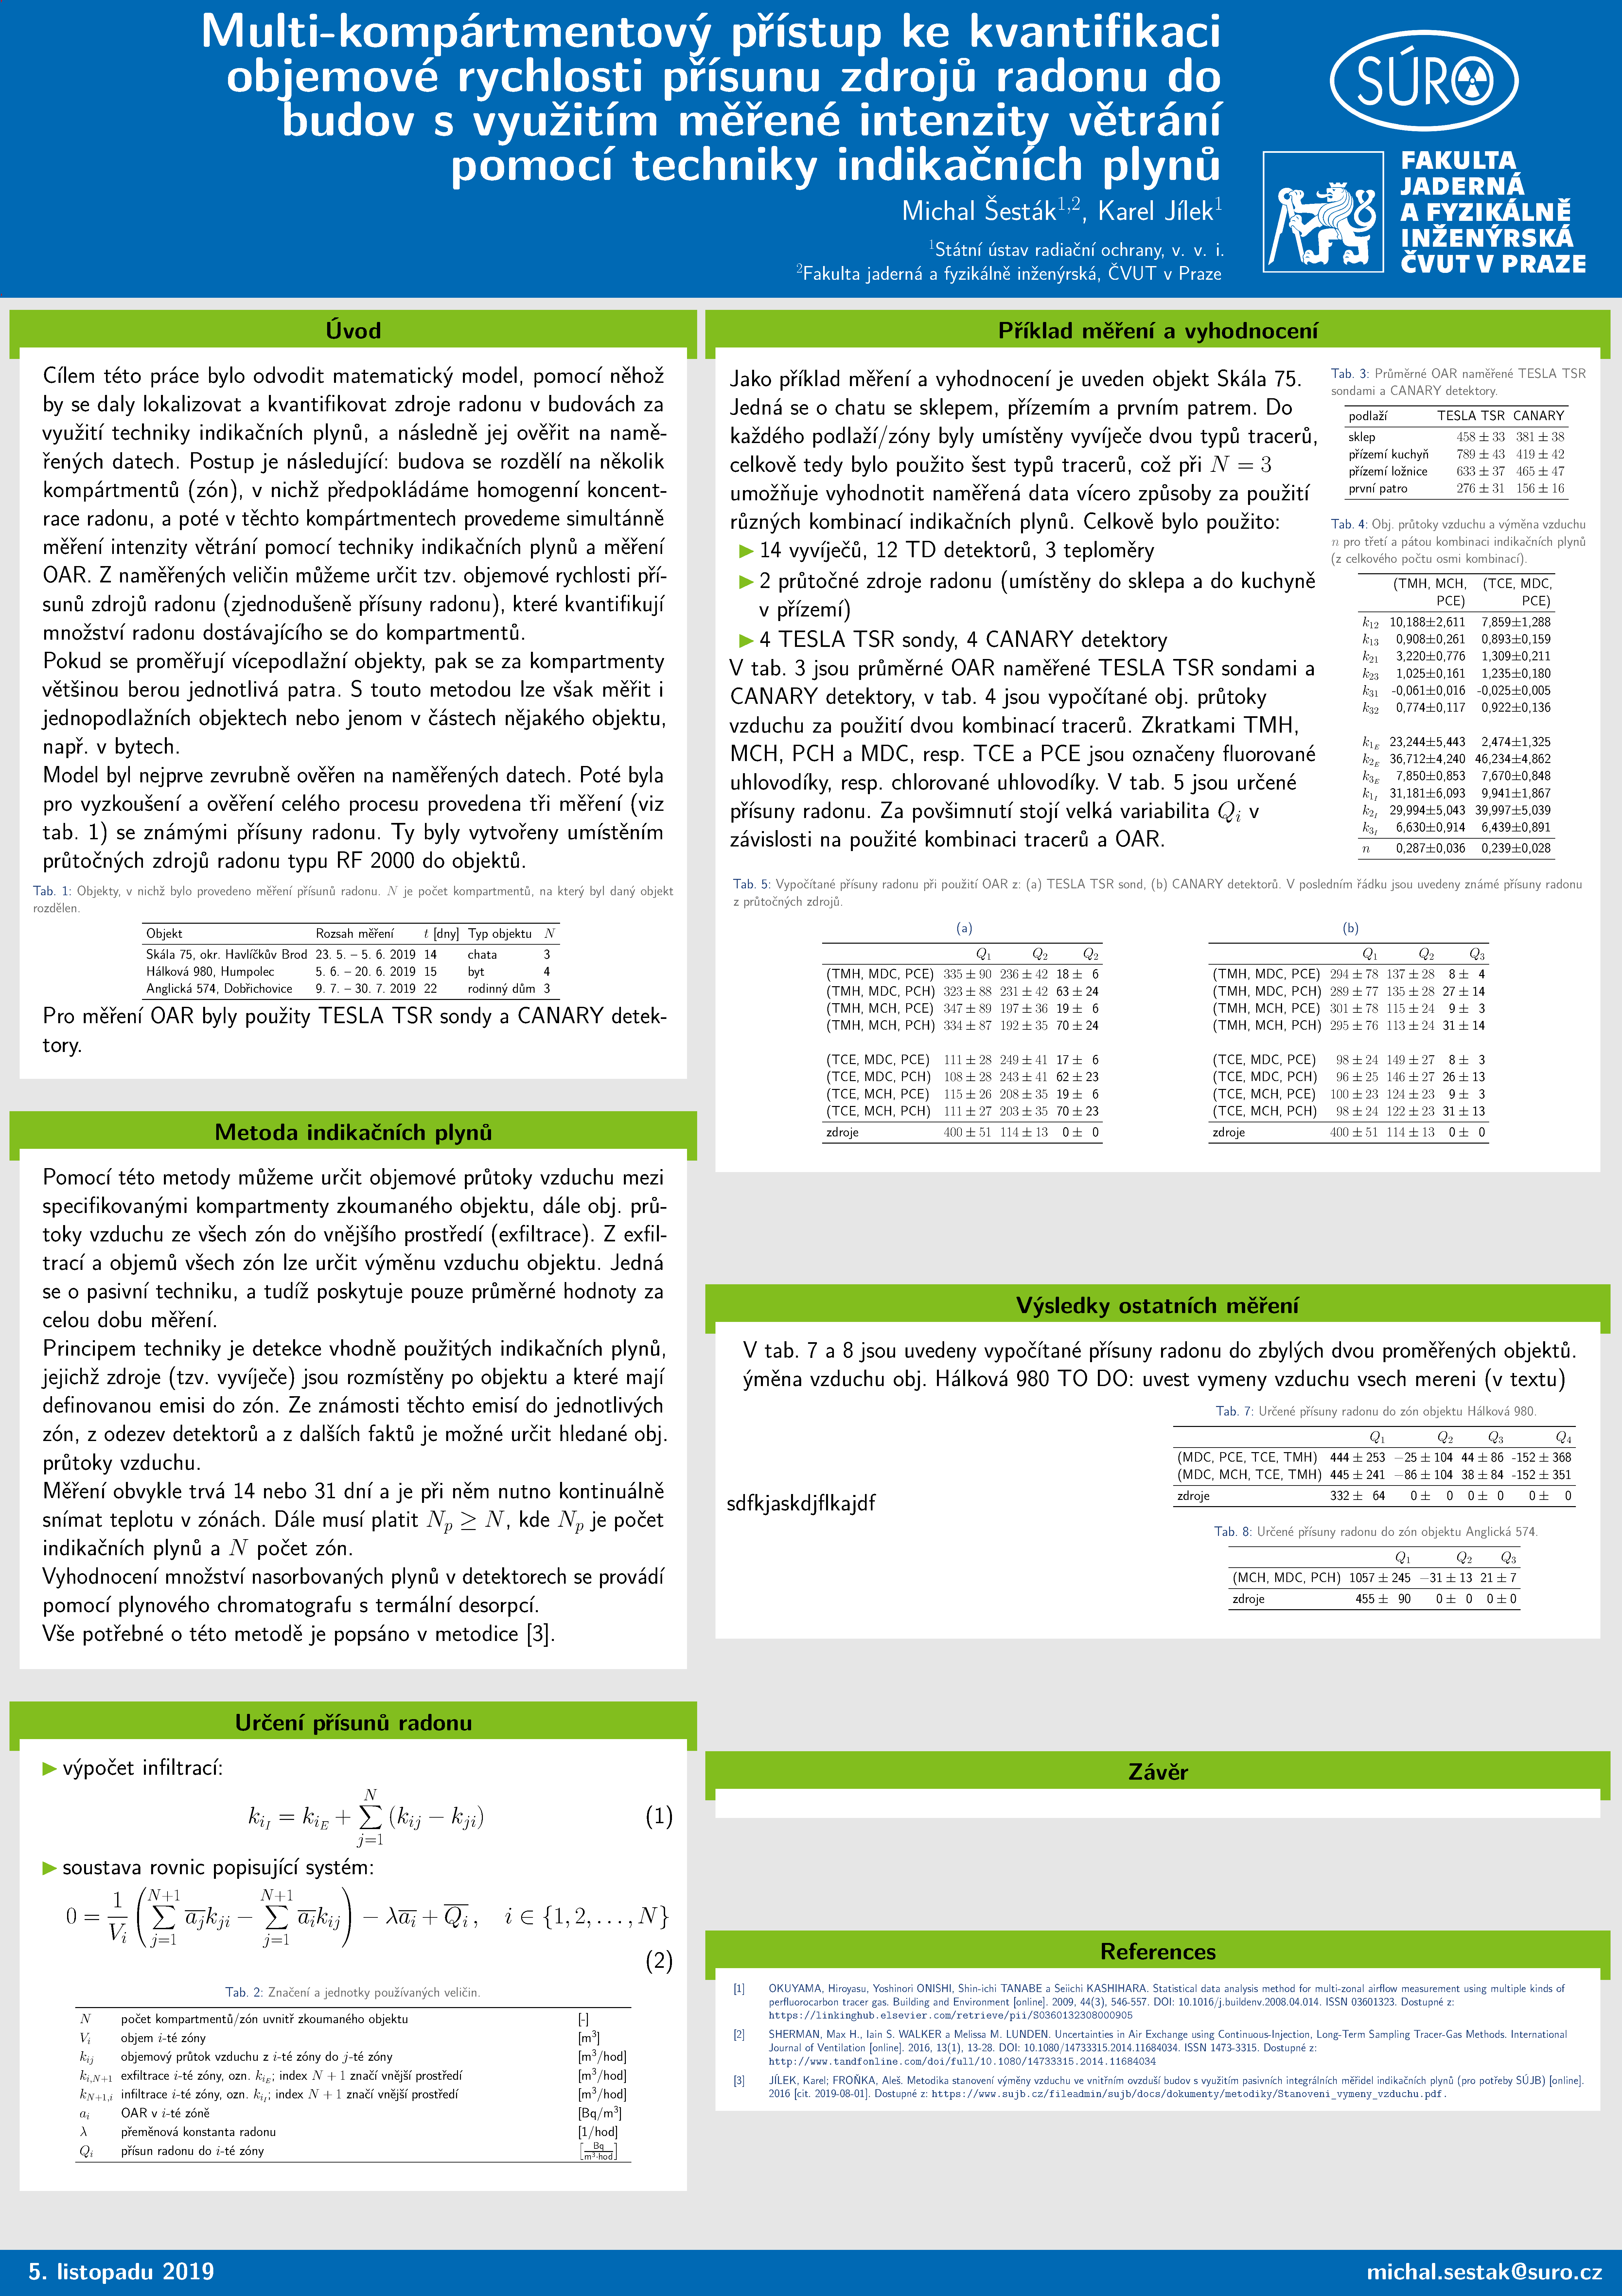
\includegraphics[height=1.05\textheight]{poster.pdf}}

% různá nastavení
%\metroset{sectionpage=simple,none}
%\begin{overlayarea}{\textwidth}{\textheight}\end{overlayarea}


\end{document}



